\section{System Overview}

The system is built around an I/O control unit that organizes all data movement
on board. Analog audio signals enter the system through a minijack and gets
routed to the hardware accelerator by the I/O controller for audio manipulation.
At the same time, processed audio is routed back from the accelerator and to the
output minijack.

\subsection{System Components}
\subsubsection{MCU}\label{intro:system-components-mcu}
The microcontroller unit is a Giant Gecko by Energy Micro (EFM32GG990F1024)
which is an energy friendly MCU capable of shutting down components that are not
in use. It does this by defining several levels of sleep mode where the outer
stage has everything on, and for each step inwards a new set of components are
shut off.

\missingfigure{add the fancy energy circle figure?}

This enables the MCU to keep I/O components working while shutting off the
processor unit on the chip.\todo{review, rewrite}

The MCU handles all I/O, effectively acting as the link between the FPGA and the
peripherals. Sound input is either gathered from a file on the SD-card or as a
stream from the audio-in jack on the board, and then passed on to the FPGA. In
addition, it is the unit controlling the FPGA, through writing the the
instructions memory each processing core contains. This, provides a simple way
in which to change the FPGA behavior.

\subsubsection{FPGA}
The FPGA is programmed with a MIMD architecture design, with the purpose of
enabling task parallelism. While this improves performance, it comes at the cost
of a more complex process architecture, which in turn increases the size of each
core. This limits the number of cores available on the FPGA, but we were able to
comfortably fit 8 cores, which is enough to implement the sound-manipulating
filters we want.

\begin{figure}[H]
    \centering
    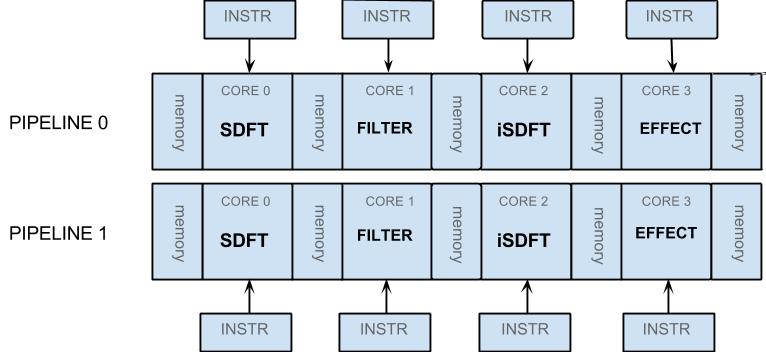
\includegraphics[height=150px]{figures/fpga/system_components_general_pipeline.png}
    \caption{A figure giving overview on how the different cores run
different programs/transforms/effects in parallel on the FPGA processing cores.}
    \label{fig:general_pipeline}
\end{figure}

Since sound processing often requires fourier transforms, several solutions were
considered for how to implement hardware support for this.

Designing a core specifically for doing the fourier transform and its inverse
was considered, but would cause increased complexity when designing the audio
processing pipelines. A variant of this idea was to equip the first and the last
core of each audio pipeline with instructions accelerating the most computing
intensive parts of the fourier transforms, but this would cause the processors
to not be homogenous.

In the end, implementing a simple floating point unit in each of the cores
would not only allow acceleration of the fourier transforms, but also
manipulation of the resulting samples in the frequency domain.

\subsubsection{Memory}
The MCU has an internal memory of 128KByte, which is not sufficient for working
comfortably with audio files loaded from the SD-card, so the decision was made
to add more memory onto the board. In addition, if something were to go wrong
with the audio-in channel and SD-card, having extra memory can work as a third
option for storing input.

\subsubsection{I/O}
Adding input and output interfaces makes handling data easier as we do not have
to go though the debug interface to insert and fetch data from the chip. Thus,
we decided to add the following components to the board.

\begin{enumerate}
	\item Micro USB connection
	\item Micro SD memory card reader
	\item Minijack sound connections
	\item Buttons and LEDs
\end{enumerate}

\paragraph{Micro USB and Micro SD}
The Micro USB was implemented with respect to energy efficiency. If we could get
the whole project to run on the power supplied by a regular USB connection, we
would have reached a low level of energy consumption. The Micro SD card was
added as mentioned earlier in the subsection\ref{intro:system-components-mcu}.

\paragraph{Minijacks}
We added two jack channels, one for input and one for output, since taking input
from a recording or playback device is much easier if you can just plug it in
rather than having to transfer data through a debugging interface. The same also
goes for output.

\paragraph{Buttons and LEDs}
The buttons and LEDs were added for ease of controlling/reading what is
happening on the PCB. We have two reset buttons for the FPGA and USB, and five
general purpose ones which the MCU controls. There's also eight LEDs, where
three are for status indications, and five are general purpose for the MCU to
control.
